\documentclass[12pt,a4paper,oneside]{report}
\usepackage[utf8]{inputenc}
\usepackage[english,russian]{babel}
\usepackage{amsmath}
\usepackage{amssymb}
\usepackage{listings}
\usepackage{geometry}
\usepackage{titlesec, blindtext, color}
\usepackage{tabularx}
\usepackage{multirow}
\usepackage{subcaption}
\usepackage{tikz,pgfplots}
\usepackage{xcolor}
\usepackage{pythonhighlight}

\geometry{pdftex, left = 2cm, right = 2cm, top = 2.5cm, bottom = 2.5cm}

% Для листинга кода:
% \lstset{ %
% 	language=c++,                 % выбор языка для подсветки (здесь это С)
% 	basicstyle=\small\sffamily, % размер и начертание шрифта для подсветки кода
% 	numbers=left,               % где поставить нумерацию строк (слева\справа)
% 	numberstyle=\tiny,           % размер шрифта для номеров строк
% 	stepnumber=1,                   % размер шага между двумя номерами строк
% 	numbersep=5pt,                % как далеко отстоят номера строк от подсвечиваемого кода
% 	showspaces=false,            % показывать или нет пробелы специальными отступами
% 	showstringspaces=false,      % показывать или нет пробелы в строках
% 	showtabs=false,             % показывать или нет табуляцию в строках
% 	frame=single,              % рисовать рамку вокруг кода
% 	tabsize=2,                 % размер табуляции по умолчанию равен 2 пробелам
% 	captionpos=t,              % позиция заголовка вверху [t] или внизу [b] 
% 	breaklines=true,           % автоматически переносить строки (да\нет)
% 	breakatwhitespace=false, % переносить строки только если есть пробел
% 	escapeinside={\#*}{*)}   % если нужно добавить комментарии в коде
% }

\lstset{  frame=single,   tabsize=2,
    breaklines,
    numbers=left,
    numberstyle={\footnotesize},
    extendedchars=\true,
    keepspaces=true
}

\titleformat{\chapter}[hang]{\Huge\bfseries}{\thechapter. \hsp}{0pt}{\Huge\bfseries}
\setcounter{tocdepth}{4} % фикс переноса 

\begin{document}
\thispagestyle{empty}
\noindent \begin{minipage}{0.15\textwidth}
	
\includegraphics[width=\linewidth]{b_logo}
\end{minipage}
\noindent\begin{minipage}{0.9\textwidth}\centering
	\textbf{Министерство науки и высшего образования Российской Федерации}\\
	\textbf{Федеральное государственное бюджетное образовательное учреждение высшего образования}\\
	\textbf{«Московский государственный технический университет имени Н.Э.~Баумана}\\
	\textbf{(национальный исследовательский университет)»}\\
	\textbf{(МГТУ им. Н.Э.~Баумана)}
\end{minipage}
\noindent\rule{18cm}{3pt}
\newline\newline
\noindent ФАКУЛЬТЕТ $\underline{\textbf{«ИНФОРМАТИКА И СИСТЕМЫ УПРАВЛЕНИЯ»}}$ \newline\newline
\noindent КАФЕДРА $\underline{\textbf{«ПРОГРАММНОЕ ОБЕСПЕЧЕНИЕ ЭВМ И ИНФОРМАЦИОННЫЕ }}$\newline\newline $\underline{\textbf{ТЕХНОЛОГИИ»(ИУ7)}}$\newline\newline
\noindent НАПРАВЛЕНИЕ ПОДГОТОВКИ $\underline{\textbf{09.03.04 ПРОГРАММНАЯ ИНЖЕНЕРИЯ}}$\newline\newline\newline\newline\newline\newline\newline
\begin{center}
    \begin{flushright}
    \Large\textbf{РАСЧЕТНО-ПОЯСНИТЕЛЬНАЯ ЗАПИСКА}\newline
	\Large\textbf{К КУРСОВОМУ ПРОЕКТУ}\newline
	\Large\textbf{НА ТЕМУ:}\newline
	\Large\textbf{«Разработка чат-бота на платформе Telegram с интеграцией базы данных 
для управления событиями»}\newline
	\end{flushright}
\end{center}
\noindent\textbf{} $\underline{\text{}}$\newline\newline\newline\newline

\begin{tabular}{lcp{5em}lp{2em}l}
	\noindent\textbf{Студент} &  $\underline{\text{ИУ7-66Б~~}}$ &             &\hspace{1cm} & & $\underline{\text{Д.А.Мокеев~}}$ \\\cline{4-3}
	 & (Группа) & &(Подпись,дата)  & & (И.О.Фамилия) \\
	 & & & & &\\
	\noindent\textbf{Руководитель} & \textbf{курсового} &  \textbf{проекта}&\hspace{1cm} & &$\underline{\text{О.В.Кузнецова~}}$ \\\cline{4-3} 
	 &  & & (Подпись,дата)  & &(И.О.Фамилия) \\
    \end{tabular}

\begin{center}
	\vfill
	Москва, \the\year
\end{center}
\newpage

\begin{center}
    \section*{Реферат}
\end{center}

\quad Курсовой проект представляет собой веб-приложение, предоставляющее функциональность для поиска пива.

Ключевые слова: web-приложение, SQLight, PeeWee, Telegram, ORM.

Приложение реализовано на языке программирования Python.

Отчёт содержит 28 страниц, 15 рисунков, 5 таблиц, 13 источников.

\clearpage
\renewcommand*\contentsname{Содержание}
\tableofcontents
\setcounter{page}{4}
\newpage

\addcontentsline{toc}{chapter}{Введение}
\chapter*{Введение}
\quad Звонки по телефону поколение Z не любит больше всего. Чтобы ориентироваться на так называемых зумеров как на целевую аудиторию необходима выработка альтернативных способов коммуникации с целью поддержания связи с клиентами. Представим бар, проводящий большое количество мероприятий. Место популярное и на мероприятия приходит много человек, но для всех вместимости не хватает. Одно из возможных решений – регистрация на эти события. Для этого можно предложить много решений – звонки, сообщения в инстаграме, разработка сайта или чат-бот. Целью данного курсового проекта является разработка чат-бота на платформе мессенджера Telegram с подключением базы данных. Задачей чат-бота является осуществлять запись гостей на мероприятия. Все запросы пользователей должны обрабатываться с использованием базы данных.

Чат-бот должен предоставлять следущий функционал:
\begin{itemize}
    \item Для клиентов – выбрать ближайшие доступные события и зарегистироваться на них
    \item для администраторов - управлять событиями, а именно добавлять новые, изменять названия, даты и время проведения, описание и другое, отменять и возвращать к возможности записи.
    \item для обоих ролей - регистирвоаться, управлять настройками своего аккаунта, получать справочную информацию.
\end{itemize}

При этом интерфейс должен быть спроектирован просто и понятно, но при этом поддерживать безболезненное добавление новых элементов для обоих ролей пользоватлей.

Для достижения цели поставлены следующие задачи:
\begin{enumerate}
    \item Анализ существующих СУБД, выбор СУБД для этого проекта;
    \item проектирование программного обеспечения;
    \item описать структуру базы данных, включая объекты, из которых она состоит;
    \item спроектировать приложение для доступа к БД;
    \item разработать приложение, которое позволит добавлять и использовать данные;
    \item тестирование приложения
\end{enumerate}


\clearpage

\chapter{Аналитическая часть}
\quad В данном разделе будут рассмотрены постановка задачи, общие сведения о БД и СУБД.

\section{Постановка задачи}

\quad В соответствии с техническим заданием на курсовой проект необходимо разработать приложение, позволяющее работать с событиями для гостей и администаторов. Для программного обеспечения выдвигаются следующие требования:
\begin{itemize}
    \item Необходимо разработать чат-бота на платформе мессенджера Telegram с подключением базы данных, то есть, необходимо реализовать две составляющие: бота(приложение) и базу данных;
    \item задачей чат-бота является предоставления сервиса клиентам и сотрудникам бара. То есть, программа должна исполнять свою основную задачу, а также необходима корректная работа программы;
    \item все запросы должны обрабатываться с использованием базы данных. То есть, должны быть разработаны запросы к базе данных;
    \item чат-бот должен иметь следующие функции:
    \begin{itemize}
        \item Для клиентов –
        \begin{itemize}
            \item просмотр событий на текущей неделе;
            \item запись на событие;
            \item отмена записи на событие;
        \end{itemize}
        \item Для администраторов –
        \begin{itemize}
            \item просмотр статистики по регистрациям;
            \item добавление новых событий;
            \item редактирование существующих событий;
        \end{itemize}
        \item Для обеих ролей –
        \begin{itemize}
            \item регистрацию нового пользователя;
            \item возможность смены имени.
        \end{itemize}
    \end{itemize}
    \item архитектура приложения и разработанный UI должны быть понятны и открыты к возможным будущим изменениям.
\end{itemize}

\section{Общие сведения о БД и СУБД}
\quad База данных — совокупность взаимосвязанных данных некоторой предметной области, хранимых в памяти ЭВМ и организованных таким образом, что эти данные могут быть использованы для решения многих задач многими пользователями. \cite{lection}.

Система управления базами данных (СУБД) – комплекс программно-языковых средств, позволяющих создать базы данных и управлять данными. СУБД — набор программ, позволяющий организовывать, контролировать и администрировать базы данных. Большинство сайтов не могут функционировать без базы данных, поэтому СУБД используется практически повсеместно. \cite{subd}.

\subsection{Основные функции СУБД}
\quad Основными функциями СУБД являются:
\begin{itemize}
    \item управление данными во внешней памяти;
    \item управление данными в оперативной памяти с использованием дискового кэша;
    \item журнализация изменений, резервное копирование и восстановление базы данных после сбоев;
    \item поддержка языков БД.
\end{itemize}

\subsection{Классификация СУБД по модели данных}
\quad Модель данных — это абстрактное, самодостаточное, логическое определение объектов, операторов и прочих элементов, в совокупности составляющих абстрактную машину доступа к данным, с которой взаимодействует пользователь. Эти объекты позволяют моделировать структуру данных, а операторы — поведение данных\cite{deit}.\\

Существует 3 основных типа моделей организации данных:
\begin{itemize}
    \item иерархическая;
    \item сетевая;
    \item реляционная.
\end{itemize}

\subsubsection{Иерархическая модель}
\quad Иерархическая модель - самая ранняя модель представления сложной структуры данных. Информация в иерархической базе организована по принципу древовидной структуры, в виде отношений «предок-потомок».

Каждая запись может иметь не более одной родительской записи и несколько подчиненных. Связи записей реализуются в виде физических указателей с одной записи на другую. Основной недостаток иерархической структуры базы данных — невозможность реализовать отношения «многие-комногим», а также ситуации, когда запись имеет несколько предков.

Графически такую структуру можно изобразить в виде дерева, состоящего из объектов различных уровней. Верхний уровень занимает один объект, второй — объекты второго уровня и так далее.

Между объектами существуют связи, каждый объект может включать в себя несколько объектов более низкого уровня. Такие объекты находятся в отношении предка (объект более близкий к корню) к потомку (объект более низкого уровня), при этом возможно, чтобы объект-предок не имел потомков или имел их несколько, тогда как у объекта-потомка обязательно только один предок. Объекты, имеющие общего предка, называются близнецами\cite{ierarh}.\\

На рисунке \ref{ris:rarh} представлена структура иерархической модели данных.
\begin{figure}[h]
	\centering
	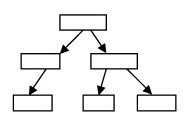
\includegraphics[scale=1]{1.png}
	\caption{Структура иерархической модели данных}
	\label{ris:rarh}
\end{figure}

\subsubsection{Сетевая модель}
\quad В сетевой структуре любой элемент может быть связан с любым другим элементом, и каждый из элементов может являться входом в структуру. Данные в сетевой модели представлены в виде совокупностей записей, а связи – в виде наборов. Сетевая модель является обобщением иерархической модели.

Сетевую структуру также можно описать с помощью исходных и порожденных элементов: каждый элемент может иметь как несколько порожденных, так и несколько исходных элементов. В ней порожденные элементы располагаются ниже исходных. В простых сетевых структурах между парой элементов поддерживается отношение «один – ко – многим». Направление и характер связи между элементами не является очевидным, и поэтому направление связи должно быть указано\cite{seti}.

Главным недостатком сетевой модели данных являются жесткость и высокая сложность схемы базы данных, построенной на основе этой модели. Так как логика процедуры выбора данных зависит от физической организации этих данных, эта модель не является полностью независимой от приложения.\\

На рисунке \ref{ris:set} представлена структура сетевой модели данных.
\begin{figure}[h]
	\centering
	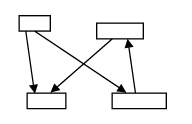
\includegraphics[scale=1]{2.png}
	\caption{Структура сетевой модели данных}
	\label{ris:set}
\end{figure}

\subsubsection{Реляционная модель}
\quad Реляционная модель базируется на теоретико-множественном понятии отношения. В математических дисциплинах существует понятие «отношение» (relation), физическим представлением которого является таблица.

Отсюда и произошло название модели – реляционная. Применительно к БД понятия «реляционная БД» и «табличная БД» являются синонимами. Реляционные базы получили наибольшее распространение в мире. Почти все продукты БД, созданные с конца 70-х годов, являются реляционными. В 1970 году появились работы, в которых обсуждались возможности применения различных табличных моделей данных. Наиболее значительной из них была статья сотрудника фирмы IBM Э.Кодда, где впервые был применен термин "реляционная модель данных". Проект System R был разработан в исследовательской лаборатории корпорации IBM. Этот
проект был задуман с целью доказать практичность реляционной модели.
 
Реляционная модель данных является совокупностью данных и состоит из набора двумерных таблиц. При табличной организации отсутствует иерархия элементов. Таблицы состоят из строк – записей и столбцов – полей. На пересечении строк и столбцов находятся конкретные значения. Для каждого поля определяется множество его значений. За счет возможности просмотра строк и столбцов в любом порядке достигается гибкость выбора подмножества элементов. Реляционная модель является удобной и наиболее широко используемой формой представления данных\cite{rel}.\\

На рисунке \ref{ris:rel} представлена структура реляционной модели данных.
\begin{figure}[h]
	\centering
	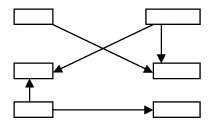
\includegraphics[scale=1]{3.png}
	\caption{Структура реляционной модели данных}
	\label{ris:rel}
\end{figure}

В результате анализа моделей баз данных, в соответствии с поставленной задачей, оптимальным решением является использование реляционной модели базы данных, так как это позволит реализовать поставленные цели, не усложняя программную архитектуру.

\section{Анализ алгоритмов работы чат-бота}
Чат-бот должен справляться со всеми задачами, описанными во введении посредством отправки вопросов, получения ответов на них и обработки полученной информации. Для обработки сообщений пользователей ботами на платформе мессенджера Telegram существует два вида алгоритмов: Webhooks — алгоритмы, работающие на основе механизмов оповещения системы о новых событиях и Long Polling — алгоритмы, работающие на основе опрашиваемых операций. Вне зависимости от используемого алгоритма все данные приходят в виде json-объектов, которые очень удобно обрабатывать.
Данные алгоритмы будут рассмотрены ниже, после чего будет выбран наиболее подходящий для решения текущей задачи.

\subsection{Long Polling — алгоритм опрашиваемых операций}
Это самый распространенный и просто реализуемый алгоритм, который используется при написании чат-ботов на платформе Telegram.
Суть этого алгоритма заключается в том, что бот периодически запрашивает обновления у Telegram, используя метод getUpdates \cite{telegram}, запрос должен отправляться не реже чем 1 раз в сутки, потому что дольше обновления не хранятся на серверах Telegram. 
В этом алгоритме важно сбалансировать скорость ответа бота и ресурсы, затрачиваемые на опрос серверов Telegram.
Если слишком часто запрашивать обновления, скорость ответа будет высокой, но будет обрабатываться много бесполезных обновлений, не содержащих никакой новой информации. Если запрашивать обновления редко, будет очень большая задержка между отправкой сообщения пользователя и ответом бота. 

\subsection{Webhooks — алгоритм оповещения системы о событиях}
В этом алгоритме нет необходимости для бота опрашивать серверы Telegram. Вместо этого сервера Telegram сообщают об обновлениях боту путем отправки в http-запросах структур данных, содержащих информацию о новых сообщениях. Webhook-и очень удобны, но также сложны в реализации. Для того, чтобы использовать этот алгоритм нужно иметь место на хостинге и зарегистрированный интернет домен. Кроме того, хостинг должен поддерживать протокол https и SSL-сертификат.

\section{Обоснование выбора алгоритма чат-бота}
Для данного курсового проекта алгоритм long polling будет более подходящим, потому как будет происходить обработка исключительно текстовых данных, а также для его использования нет необходимости регистрировать интернет домен, с этим алгоритмом бота можно развернуть со своего компьютера. В данном проекте основной задачей остается реализация базы данных, поэтому можно пренебречь скоростью обработки сообщений.

\section*{Вывод}
\quad В данном разделе были рассмотрены постановка задачи, общие сведения о БД и СУБД и алгоритм работы чат-ботов



\chapter{Конструкторская часть}
\qquad В данном разделе будет рассмотрено проектирование ПО, представлены диаграмма вариантов использования, ER диаграмма и диаграмма базы данных. Рассмотрена регистрация и аутентификация пользователей. 

Необходимо создать модель работы системы, которая будет связывать приложение и базу данных. Все операции ввода-вывода связаны с обращением к базе данных. Обработка и получение сообщений – задача библиотеки и алгоритмов Telegram бота.
\section{Диаграмма вариантов использования}
\quad Use-case диаграмма состоит из графической диаграммы, описывающей действующие лица и конкретные действия, которые выполняет пользователь при работе с системой.
Данная диаграмма предназначена для определения функциональных требований. В системе есть три типа пользователей:
\begin{itemize}
    \item Незарегистрированный пользователь(гость): пишет команду /start – его уникальный Telegram ID сохраняется в базу данных со статусом PREGISTRADED, на этом этапе пользователю предлагается ввести имя, остальные функции не доступны; 
    \item зарегистрированный пользователь, гость: использует приложение для просмотра предстоящих событий и управления регистрацией на них, имеют тип пользователя GUEST и статус REGISTRATED; переход в режим пользователя администратор осуществляется с помощью команды /admin и требует ввода пароля;
    \item зарегистрированный пользователь, администратор: использует приложение для редактирования и создания новых событий, просмотра статистики. Имеет тип пользователя ADMIN и статус REGISTRATED. 
\end{itemize}

\quad На рисунке \ref{ris:case} представлена Use-Case диаграмма. 
\begin{figure}[h]
	\centering
	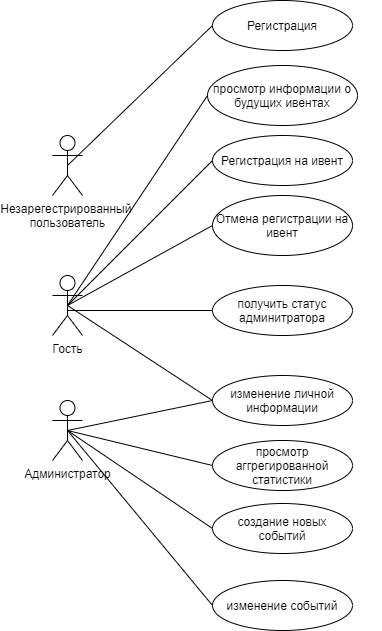
\includegraphics[scale=1.2]{UseCasediagram.png}
	\caption{Use-Case диаграмма}
	\label{ris:case}
\end{figure}
\clearpage


\section{Конструирование базы данных}
База данных включает в себя три таблицы, которые изображены на рисунке  \ref{ris:dbdiagram}
\begin{figure}[h]
	\centering
	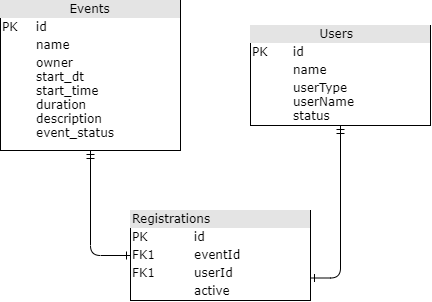
\includegraphics[scale=1.2]{diagram.png}
	\caption{Диаграмма таблиц базы данных}
	\label{ris:dbdiagram}
\end{figure}

Таблица Users хранит информацию о пользователе и имеет следующие поля:
\begin{itemize}
    \item id – идентификатор – primary key – в качестве него используется уникальный Telegram ID пользователя; 
    \item name – имя гостя или администратора;
    \item userType – тип пользователя;
    \item userName – никнейм пользователя в Telegram (@nickname)
    \item status - статус пользователя (зарегистрирован, отключен и т.д.)
\end{itemize}
Таблица Events хранит информацию о событиях и имеет следующие поля: 
\begin{itemize}
    \item id – суррогатный primary key;  
    \item name –  название события;
    \item owner – никнейм владельца события;
    \item {start\_dt} – дата проведения;
    \item {start\_time} – время начала;
    \item duration – продолжительность;
    \item description – описание;
    \item {event\_status} – статус (состоится, отменен и т.д.)
\end{itemize}

Таблица Registration хранит информацию о записях, тем самым связывая таблицы пользователей и событий, и имеет следующие поля: 
\begin{itemize}
    \item id – суррогатный primary key;    
    \item eventId – идентификатор события – внешний ключ; 
    \item userId – идентификатор пользователя – внешний ключ;
    \item status – статус регистрации (активна или отменена).
\end{itemize}

ER-диаграмма базы данных показана на рисунке \ref{ris:erdiagram} Было выделено три сущности. Сущность Appointment связана с сущностями Patient и Doctor связью один ко многим. Атрибуты сущностей также отображены на диаграмме.

\begin{figure}[h]
	\centering
	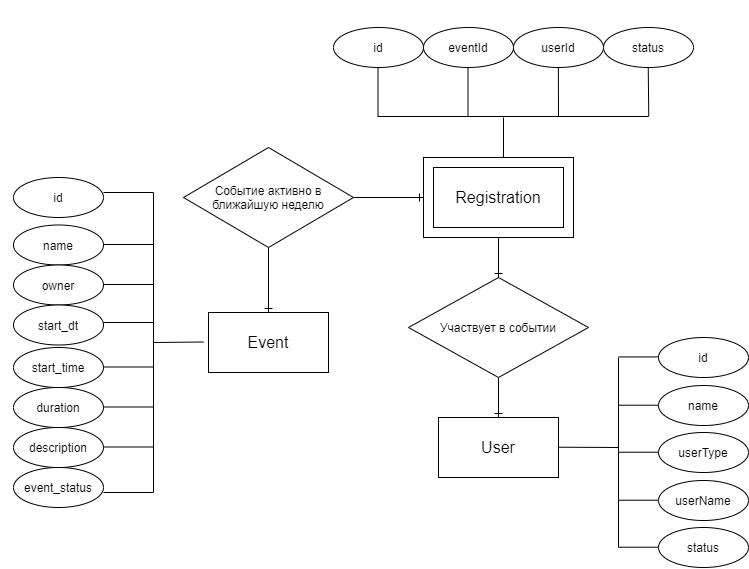
\includegraphics[scale=0.9]{ERdiagram.png}
	\caption{ER-диаграмма модели}
	\label{ris:erdiagram}
\end{figure}

\subsection{Модель системы}
Модель на вход получает сообщения от пользователя, они обрабатываются при помощи использования алгоритмов чат-бота, полученные данные, передаются в базу данных, данные, которые в последствии отправляются пользователю, тоже берутся из базы данных, приложение формирует ответное сообщение, оно отправляется пользователю при помощи библиотеки Telebot.
Обращение к базе данных происходит каждый раз, когда требуется информация о врачах, пациентах или записях.

\subsection{Структуры данных}
В данном подразделе будут рассмотрены структуры данных, которые будут использованы в программе. В структуры входят:
\begin{itemize}
    \item Объектно-реляционное отображение базы данных классами:
    \begin{itemize}
        \item Класс пользователя User;
        \item класс события Event;
        \item класс записей Registration.
    \end{itemize}
    \item Message\_handlers – механизмы, позволяющие работать с сообщениями пользователя;
    \item сallback\_query\_handlers – механизмы, позволяющие обрабатывать ввод пользователя с помощью inline buttons;
    \item классы библиотеки Telebot, содержащие информацию о сообщениях пользователя;
    \item классы клавиатур Keyboard, позволяющие выводить на экран пользователя кнопки с доступными вариантами ответов;
    \item классы констант такие как UserStatus, UserType, EventStatus и т.д.;
    \item классы GuestChoiceButton и AdminChoiceButton содержащие текстовые ответы на сообщения;
    \item статические параметры такие как dateFormat, timeFormat, API-token и т.д.
\end{itemize}

\subsection{Модель данных}
В данной работе будет использована технология ORM. ORM (англ. Object-Relational Mapping, рус. объектно-реляционное отображение) — технология программирования, которая связывает базы данных с концепциями объектно-ориентированных языков программирования, создавая «виртуальную объектную базу данных». ORM позволяет удобно интегрировать модели в приложения с объектно-ориентированным стилем программирования.

\section*{Вывод}
\quad Были представлены диаграммы вариантов использования и «сущность~— связь», с помощью которых спроектирована база данных и архитектура приложения, обеспечивающего возможность пользователей авторизовываться и аутентифицироваться, создавать, редактировать и оценивать статьи и комментарии к ним.


\chapter{Технологическая часть}
\quad В данной части рассмотрены популярные СУБД и используемый фреймворк, приведены листинги классов для оформления таблиц базы данных, доступ к данным, а также рассмотрена интерфейс приложения. 

\section{Разбор различных СУБД}

\quadДля данной задачи подойдет использование реляционной модели данных. Реляционная модель состоит из трех частей: структурной, целостностной и манипуляционной. Структурная часть реляционной модели описывает, из каких объектов состоит реляционная модель. В целостностной части реляционной модели фиксируются два базовых требования целостности, которые должны выполняться для любых отношений в любых реляционных базах данных. Это целостность сущностей и ссылочная целостность. Манипуляционная часть реляционной модели описывает два эквивалентных способа манипулирования реляционными данными – реляционную алгебру и реляционное исчисление. \cite{gavr}
Таким образом, выбранная СУБД должна поддерживать реляционную модель данных. То есть, сущности должны храниться в таблицах (структурная часть), а также сущности разных таблиц должны иметь возможность быть связанными, то есть должна присутствовать возможность выстраивать отношения между сущностями при помощи внешних ключей (целостная часть). Также должна иметься возможность управлять данными, изменять их, производить поиск по данным и так далее (манипуляционная часть).

Для разработки была выбрана реляционная модель базы данных, поэтому рассмотрим три наиболее важные и популярные СУБД с открытым исходным кодом: SQLite, MySQL, PostgreSQL.

\subsection{SQLite}

\quadSQLite - это встраиваемая файловая СУБД, которая не требует установки или настройки. Это, в свою очередь, означает, что приложение не запускается в рамках отдельного серверного процесса, который необходимо запускать, останавливать или настраивать. Такая безсерверная архитектура позволяет базе данных поддерживать кроссплатформенность.
Полная база данных SQL содержится в одном файле на диске, и все операции чтения и записи осуществляются непосредственно в этот файл на диске. Поскольку данные напрямую записываются обратно в файл диска, SQLite поддерживает систему ACID защиты транзакций от сбоев выделения памяти и ошибок ввода-вывода диска, которые могут возникнуть в результате непредвиденных сбоев системы или сбоев питания.
 \cite{sqlite}.\\

Преимущества:
\begin{itemize}
	\item[$+$] ГБиблиотека SQLite - одна из самых компактных библиотек СУБД, размер библиотеки может быть меньше 600 КБ.
	\item[$+$] База использует для работы единственный файл, что хорошо влияет на ее переносимость.
	\item[$+$] Легко настраиваема и показывает хорошие результаты на веб-сайтах с низким и средним трафиком (~ 100 тыс. Запросов в день). 
	\item[$+$] Совместима с языком программирования Python.
\end{itemize}

Недостатки:
\begin{itemize}
	\item[$-$] Отсутствие встроенного шифрования данных, что стало стандартом для предотвращения наиболее распространенных хакерских атак в интернете.
	\item[$-$] База не поддерживает систему учета пользователей, в то время как другие популярные СУБД поддерживают эту возможность.
	\item[$-$] Только одна операция записи за транзакцию, что уменьшает производительность системы
\end{itemize}

\subsection{MySQL}
\quad MySQL - одна из самых популярных и широко распространенных СУБД с открытым исходным кодом. В отличие от SQLite, она использует архитектуру клиент-сервер, которая состоит из многопоточного сервера SQL. Эта многопоточная природа MySQL обеспечивает большую производительность, поскольку потоки ядра могут легко использовать несколько процессоров. База данных написана на C и C ++ и поддерживает различные платформы. Она также придерживается системы ACID для обеспечения согласованности транзакций. \cite{sqlite}\\

Преимущества:
\begin{itemize}
	\item[$+$] Обширный функционал и наличие корпоративных функций.
	\item[$+$] Важным отличием MySQL от SQLite является поддержка многопользовательских функциями MySQL. Это и наличие корпоративных функций, делает эту СУБД идеально подходящей для распределенных приложений.
	\item[$+$] MySQL имеет преимущество перед PostgreSQL, когда речь идет о пропускной способности и производительности. Она также намного проще в установке и использовании и более широко используется в сравнению с PostgreSQL.
\end{itemize}

Недостатки:
\begin{itemize}
	\item[$-$] Плохо проявляет себя на больших операциях SELECT и BULK INSERT.
	\item[$-$] Уязвимости: метод обработки данных, применяемый в MySQL, делает эту СУБД немного менее надёжной по сравнению с другими СУБД.
	\item[$-$] Медленное развитие: хотя MySQL является продуктом с открытым исходным кодом, он очень медленно развивается.
\end{itemize}

\subsection{PostgreSQL}
\quad PostgreSQL — это продвинутая открытая объектно-ориентированная СУБД.
PostgreSQL - это СУБД с открытым исходным кодом, в которой особое внимание уделяется расширяемости и соответствию стандартам. Как и MySQL, PostgreSQL использует модель данных клиент-сервер, а процесс сервера, который обрабатывает связь с клиентом, управляет файлами и операциями базы данных, называется процессом postgres.
PostgreSQL обрабатывает параллельные клиентские сессии, «разветвляя» новый процесс для каждого соединения. Этот процесс отделен от основного процесса postgres, он создается и уничтожается во время жизненного цикла клиентского соединения. Написанный на C, Postgres также поддерживает ACID, функции и хранимые процедуры. В отличие от MySQL, PostgreSQL поддерживает материализованные представления (кэшированные представления), что ускоряет частый доступ к большим и активным таблицам. \cite{sqlite}


Преимущества:
\begin{itemize}
	\item[$+$] Благодаря превосходной способности параллельной обработки PostgreSQL выходит на первое место (по сравнению с MySQL) при выполнении длинных SELECT. 
	\item[$+$] Помимо встроенных функций, PostgreSQL поддерживает множество открытых сторонних инструментов для проектирования, управления данными и т.~п.
	Одним из таких инструментов является веб-приложение pgAdmin.
	\item[$+$] База очень хорошо масштабируется и расширяется.
	\item[$+$] Работает быстро и надежно, база способна обрабатывать терабайты данных.
	\item[$+$] PostgreSQL всегда считался лучшим для аналитических процессов, таких как хранилище данных. 
\end{itemize}

Недостатки:
\begin{itemize}
	\item[$-$] Механизм хранения PostgreSQL требует большой работы, он неоптимален в определенных случаях.
	\item[$-$] PostgreSQL очень энергоемкий в сравнении с другими СУБД. Поскольку PostgreSQL разветвляет процесс для новых клиентских соединений, это может занять до 10 МБ на соединение. Эта модель может занимать много памяти при одновременном подключении клиента по сравнению с моделью MySQL для потокового подключения.
	\item[$-$] Сложно устанавливать, много обновлений, не поддерживает кластеризованные индексы, что может оказать огромное негативное влияние на производительность по сравнению с базами данных MySQL.

\end{itemize}

В данном курсовом проекте будет использоваться PostgreSQL ввиду объективного превосходства над всеми остальными СУБД.


\section{Средства реализации}
\quad Для написания программного обеспечения для данного курсового проекта был использован язык Python 3.8. Этот язык поддерживает объектно-ориентированную модель разработки, что позволяет четко структурировать программу и легко модифицировать отдельные ее компоненты независимо от других. 
В качестве среды разработки был использован PyCharm 2020.1 (build 201.6668.115). Он обладает всем необходимым функционалом для написания, профилирования и отладки программ.
Так как серверная программа не использует много ресурсов, достаточно одного потока для её работы. 

\section{Использование объектно-реляционного отображения}
Для связывания серверной части и СУБД, было решено использовать объектно-реляционное отображение базы данных.
Объектно-реляционное отображение — это технология программирования, которая связывает базы данных с концепциями объектно-ориентированных языков программирования, создавая «виртуальную объектную базу данных». 
Чтобы использовать этот метод работы с базой данных, было решено использовать классы и методы библиотеки Peewee.
Для работы с таблицами базы данных было создано три класса — каждый класс являлся представлением таблицы на ООП. Классы представлены в листинге 3.2.1

\begin{python}
class Events(Model):
    id = AutoField(unique=True, null=False)
    name = CharField()
    owner = CharField()
    start_dt = DateField(formats=[dateFormat])
    start_time = TimeField(formats=[timeFormat])
    duration = CharField()
    description = CharField()
    event_status = IntegerField(default=None)

    class Meta:
        db_table = 'events'
        database = db
        
    class Users(Model):
    id = PrimaryKeyField(unique=True, null=False)
    name = CharField(default="")
    userType = IntegerField(-1)
    userName = CharField(default="")
    status = IntegerField(default=UserStatus.UNKNOWN)

    class Meta:
        db_table = 'users'
        database = db


class Registrations(Model):
    id = AutoField(unique=True, null=False)
    eventId = ForeignKeyField(Events, backref='events')
    userId = ForeignKeyField(Users, backref='users')
    active = IntegerField()

    class Meta:
        db_table = 'registrations'
        database = db
\end{python}

\begin{center}
    Листинг 3.2.1 – Классы пользователя, события и регистрации
\end{center}

Данные классы соответствуют описанной в конструкторском разделе базе данных. Класс Registrstion связан с классами Users и Events посредством внешних ключей (ForeignKeyField). Поля классов соответствуют полям базы данных из конструкторского раздела. Были выбраны типы данных, соответствующие данным, хранимым в этих полях.

Для обращения к базе данных были реализованы функции записи и получения данных. Добавление данных представлено в листинге 3.2.2.


\begin{python}
def add_user(id, name="", userType=UserType.UNKNOWN, userName="", status=UserStatus.UNKNOWN):
    Users.create(
        id=id,
        name=name,
        userType=userType,
        userName=userName,
        status=status
    )

    return True

# true on success
def addRegistrationOnEvent(event_id, user_id) -> bool:
    try:
        Registrations.get(Registrations.eventId == event_id,
                          Registrations.userId == user_id,
                          Registrations.active==   RegistrationStatus.ACTIVE)
    except:
        add_registration(event_id,
 user_id, RegistrationStatus.ACTIVE)
        return True

def add_registration(eventId=0, 
userId=0, active=RegistrationStatus.INACTIVE):
    app = Registrations.create(
        eventId=eventId,
        userId=userId,
        active=active
    )
    app.save()
    return True 


def add_event(name="", owner="", start_dt="", start_time="",
              duration="",
 description="", event_status=EventStatus.UNKNOWN):
    Events.create(
        name=name,
        owner=owner,
        start_dt=start_dt,
        start_time=start_time,
        duration=duration,
        description=description,
        event_status=event_status
    )

    return True

\end{python}

\begin{center}
    Листинг 3.2.2 –  Добавление записей
\end{center}

\section{Реализация доступа к данным}
\quad В листинге 3.3.1 представлены функции запросов для получения данных из таблиц. 

\begin{python}
def getTodayEvents() -> str:
    today = date.today().strftime(dateFormat)
    return selectValidEventForTheDay(today)
def selectValidEventForTheDay(day):
    todayEvents = Events.select()
                         .where(Events.start_dt==day,                   Events.event_status == EventStatus.GOINGTO)
                         .execute()
    events = []
    for line in todayEvents:
        events.append(reply_event_markup.format(
                     line.name, line.start_dt,
                     line.start_time,line.duration,
                     line.owner, line.description))
    return '\n'.join(events)

def selectEventNamesForTheDay(day, status=EventStatus.GOINGTO):
    if status != EventStatus.UNKNOWN:
        todayEvents = Events.select()
            .where(Events.start_dt==day,
                   Events.event_status== status).execute()
    else:
        todayEvents = Events.select()
                     .where(Events.start_dt == day)
                     .execute()
    events = []
    for line in todayEvents:
        event = {"id": line.id,
                 "name": line.name,
                 "start_dt": line.start_dt,
                 "status": line.event_status,
                 "owner": line.owner,
                 "description": line.description,
                 "start_time": str(line.start_time)}
        events.append(event)

    return events

def selectUserActiveRegistratedEvents(id):
    today = date.today()
    query = (Registrations
             .select(Registrations.id, Events.name, Events.id, Registrations.eventId)
             .join(Events)
             .where(Registrations.userId == id,
                    Events.start_dt.year >= today.year,
                    Events.start_dt.month >= today.month,
                    Events.start_dt.day >= today.day,
                    Registrations.active == RegistrationStatus.ACTIVE))

    events = []
    for line in query:
        event = {"id": line.id,
                 "name": line.eventId.name,
                 "eventId": line.eventId.id
                 }

        events.append(event)

    return events

\end{python}

\begin{center}
    Листинг 3.3 – Классы пользователя, события и регистрации
\end{center}


\section{Описание интерфейса чат-бота}
\quad Для начала работы пользователь должен дать команду /start (стандартное поведение для Telegram-бота), после чего ему предлагается ввести свое имя. Впоследствии имя будет использоваться для регистрации и может быть изменено программно. После введения имени пользователь получает доступ к блоку функций гостя (просмотр и регистрация на события).
 Переход пользователя к режиму администратора начинается после вызова пользователем команды /admin. Будет предложено ввести пароль (подразумевается, что он выдается сотрудникам) и в случае совпадения становятся доступны функции блока администратора — просмотр статистики, изменение и добавление новых событий. 
Оба типа пользователей имеют доступ к командам /menu — вызывает основное меню для соответствующего типа пользователя и /help — позволяет получить справочную информацию о боте и доступных командах. 


На рисунке \ref{ris:reg1}  представлена регистрация нового пользователя, основное и главное меню пользователя-гостя. На рисунке \ref{ris:todayWeek} показан интерфейс для просмотра пользователем событий - сегодня и в любой день текущей календарной недели и соответсвующий ответ бота.

\begin{figure}[h]
	\centering
	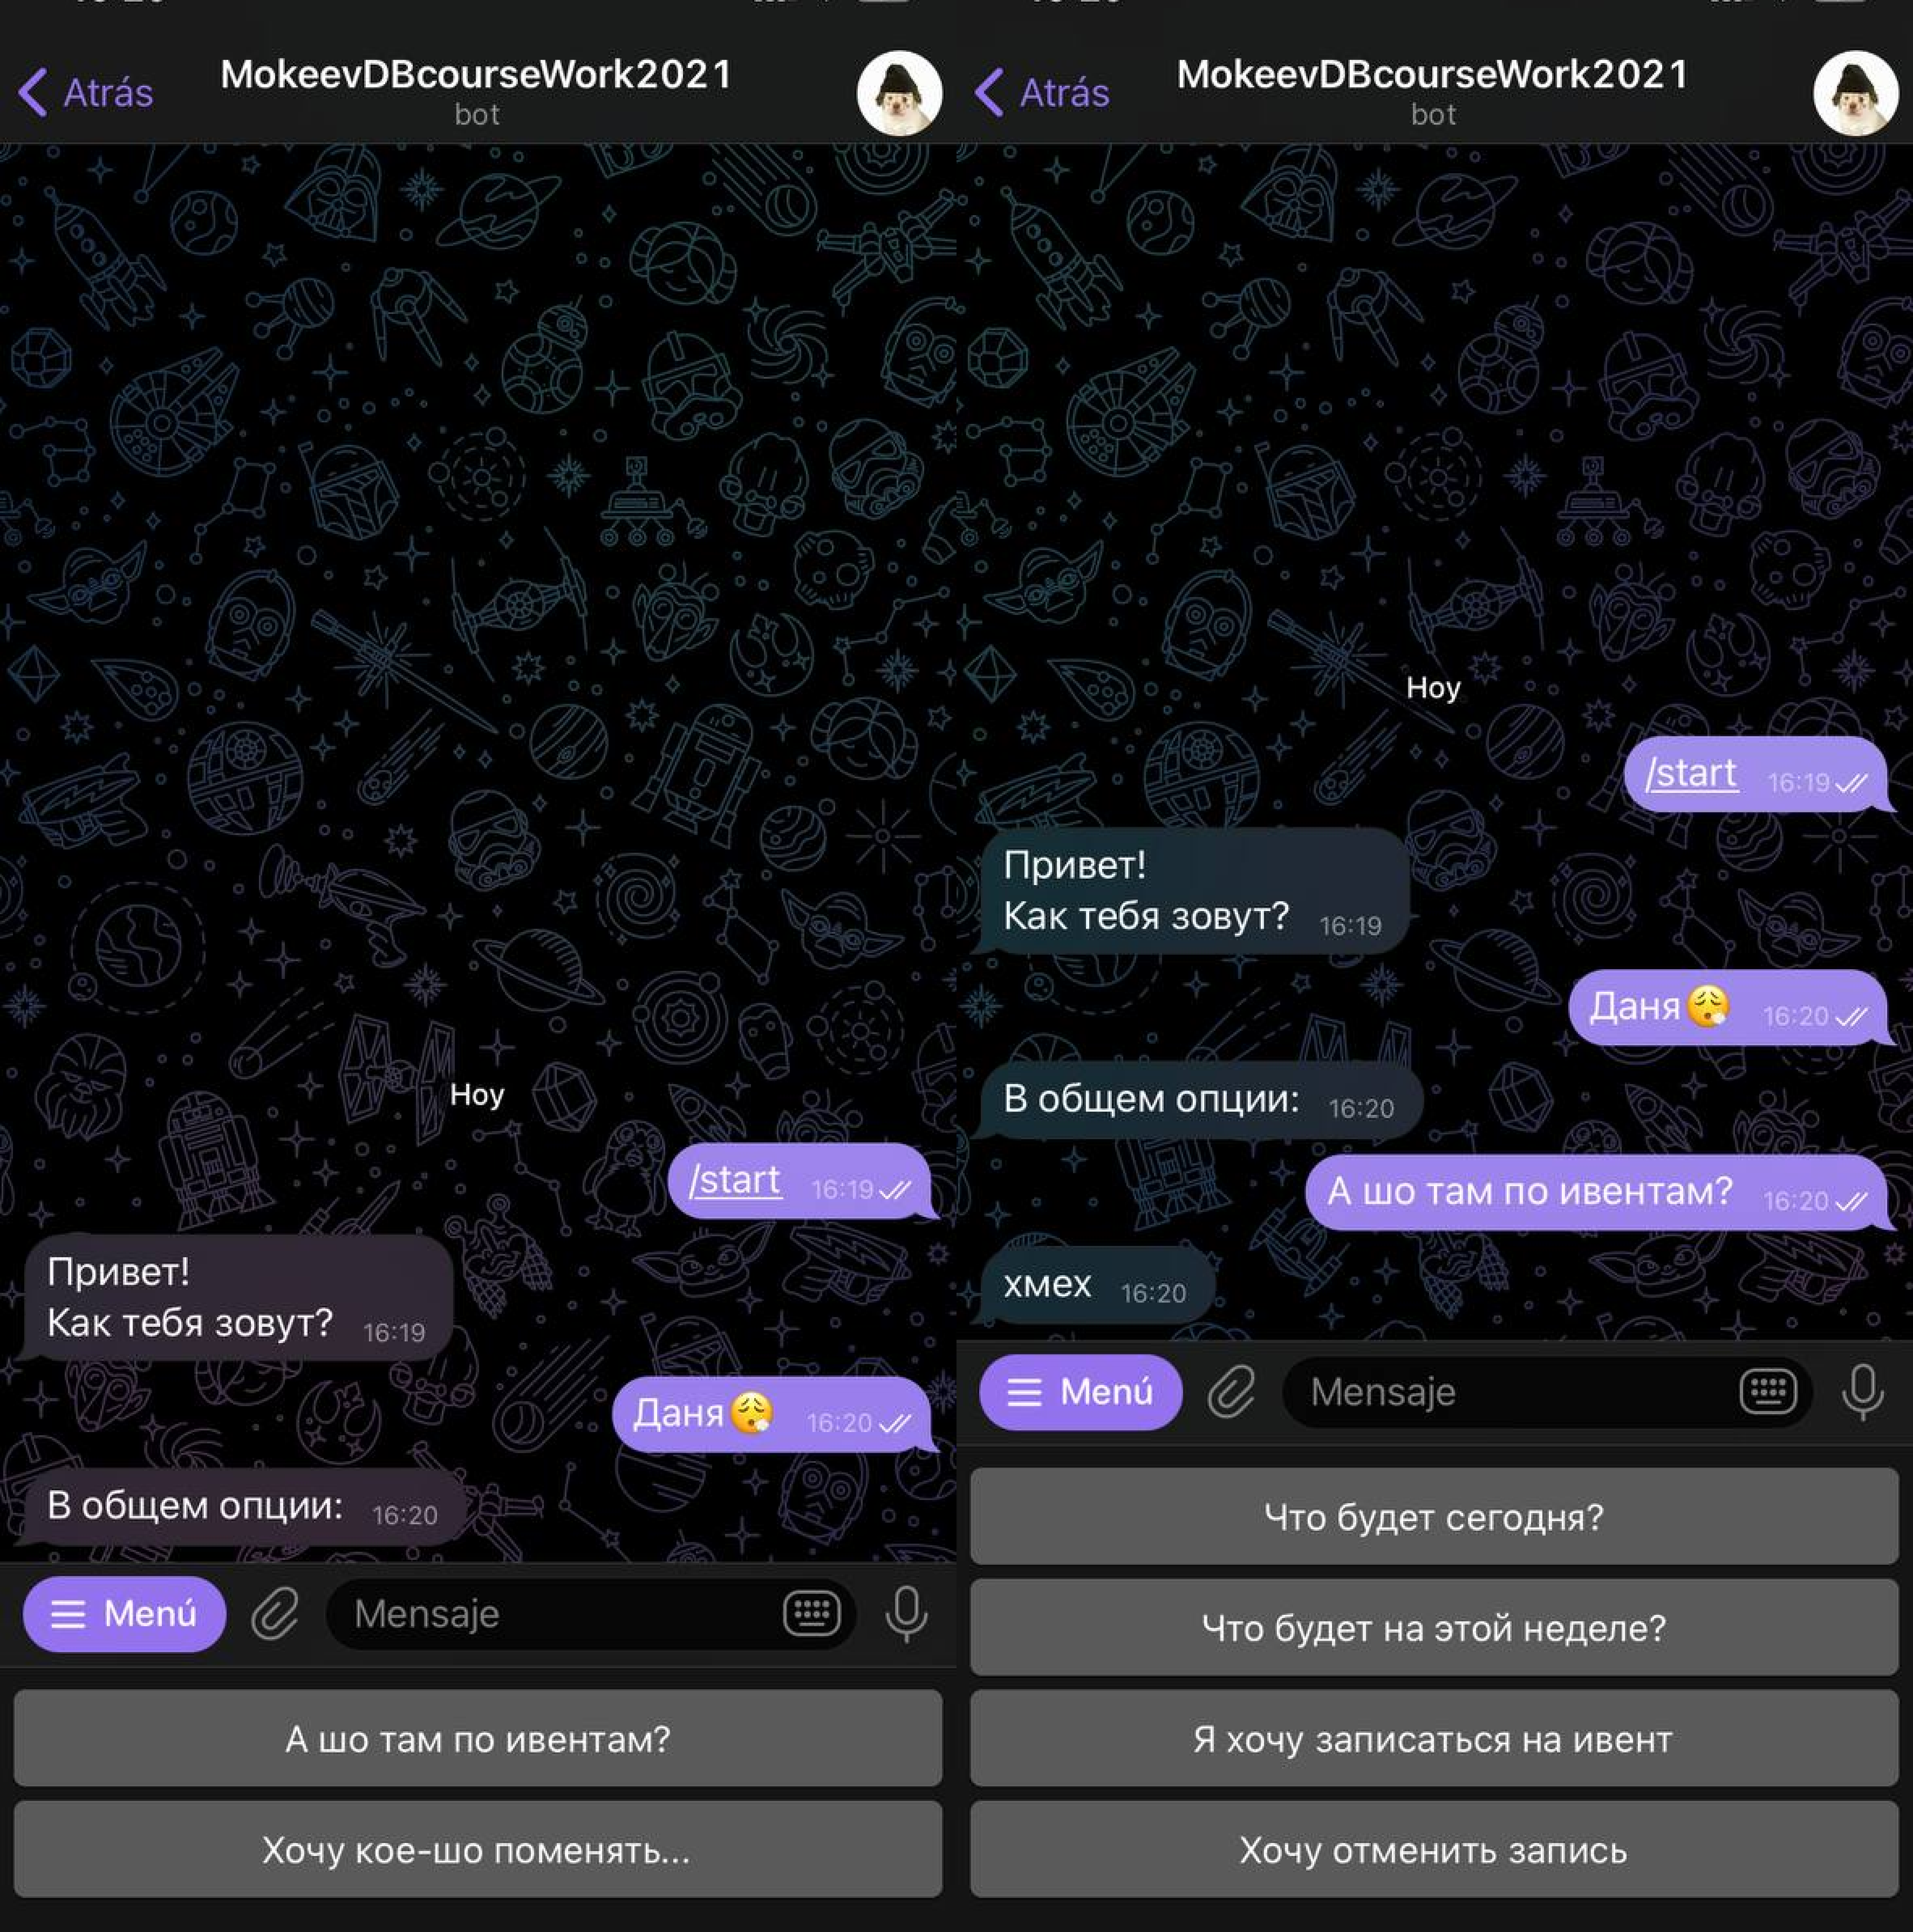
\includegraphics[scale=0.3]{regAndMainMenu.png}
	\caption{Регистрация нового пользователя, основное и главное меню Пользователя-гостя}
	\label{ris:reg1}
\end{figure}


\begin{figure}[h]
	\centering
	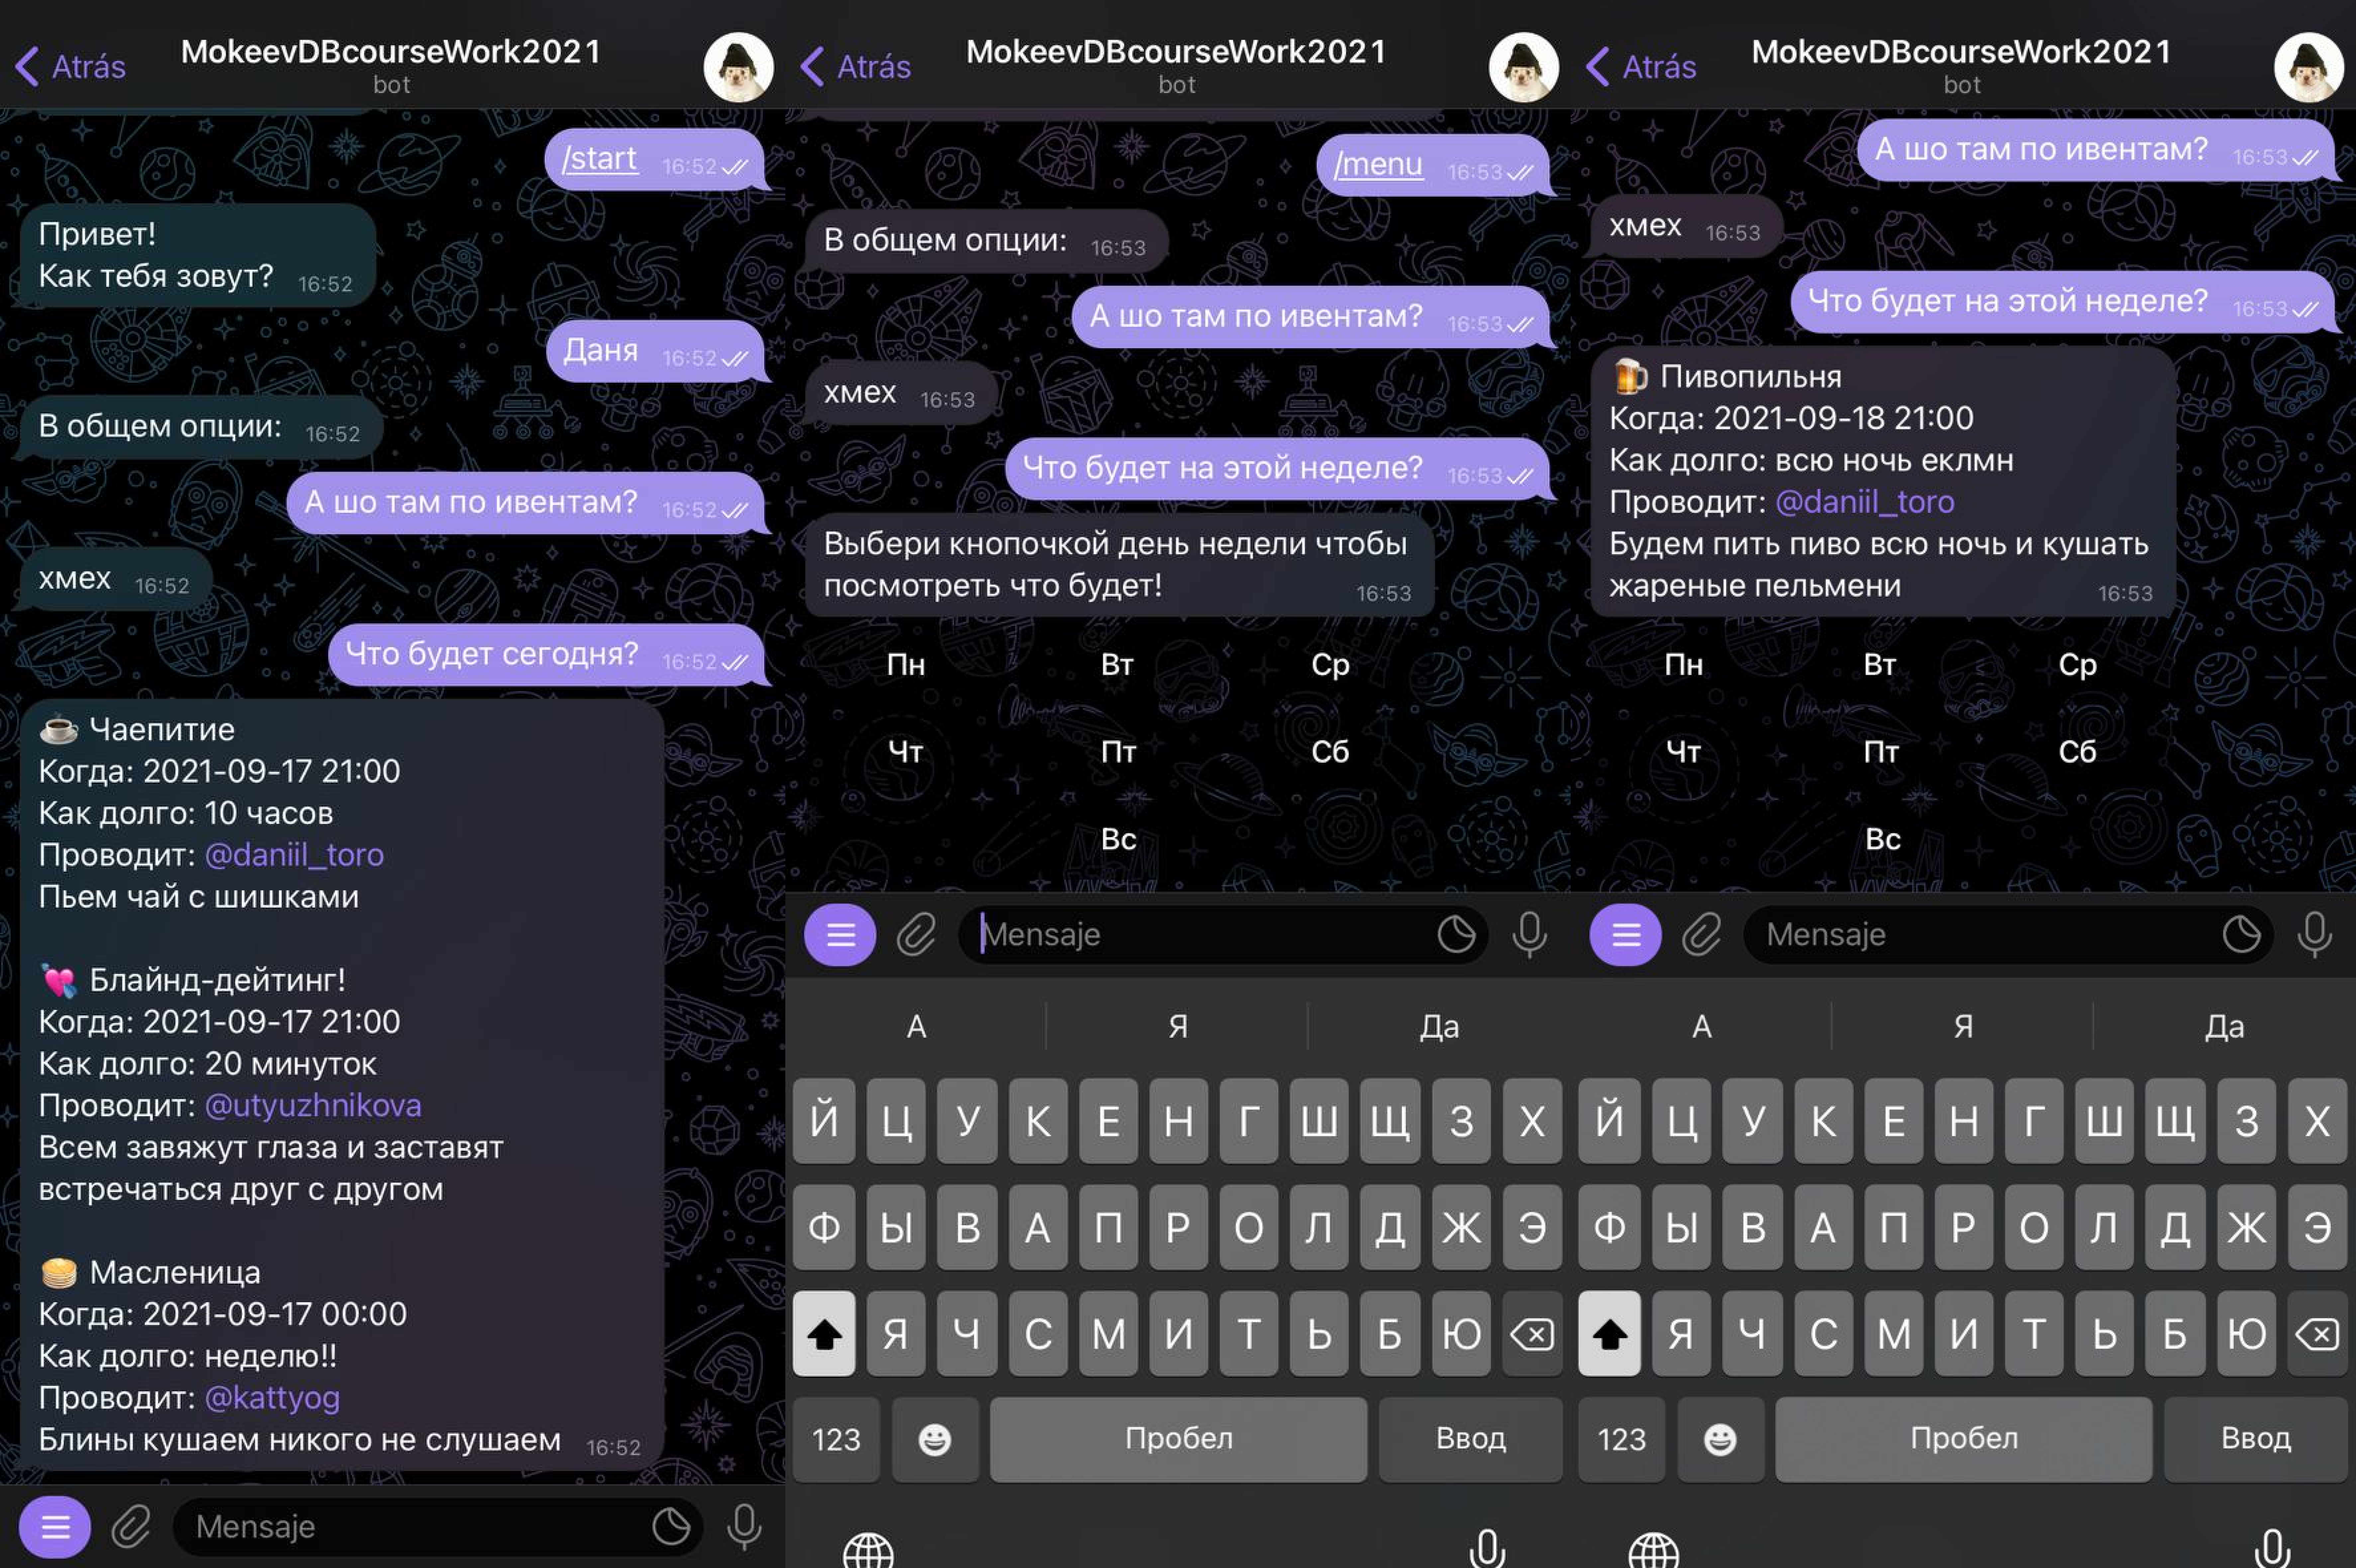
\includegraphics[scale=0.3]{showTodatWeek.png}
	\caption{Интерфейс для просмотра сегодняшего события и событий недели}
	\label{ris:todayWeek}
\end{figure}



На рисунках \ref{ris:regEvent} и \ref{ris:unregEvent} представлены интерфейс и ответы бота при регистрации и отмене регистрации пользователем. 

\begin{figure}[h]
	\centering
	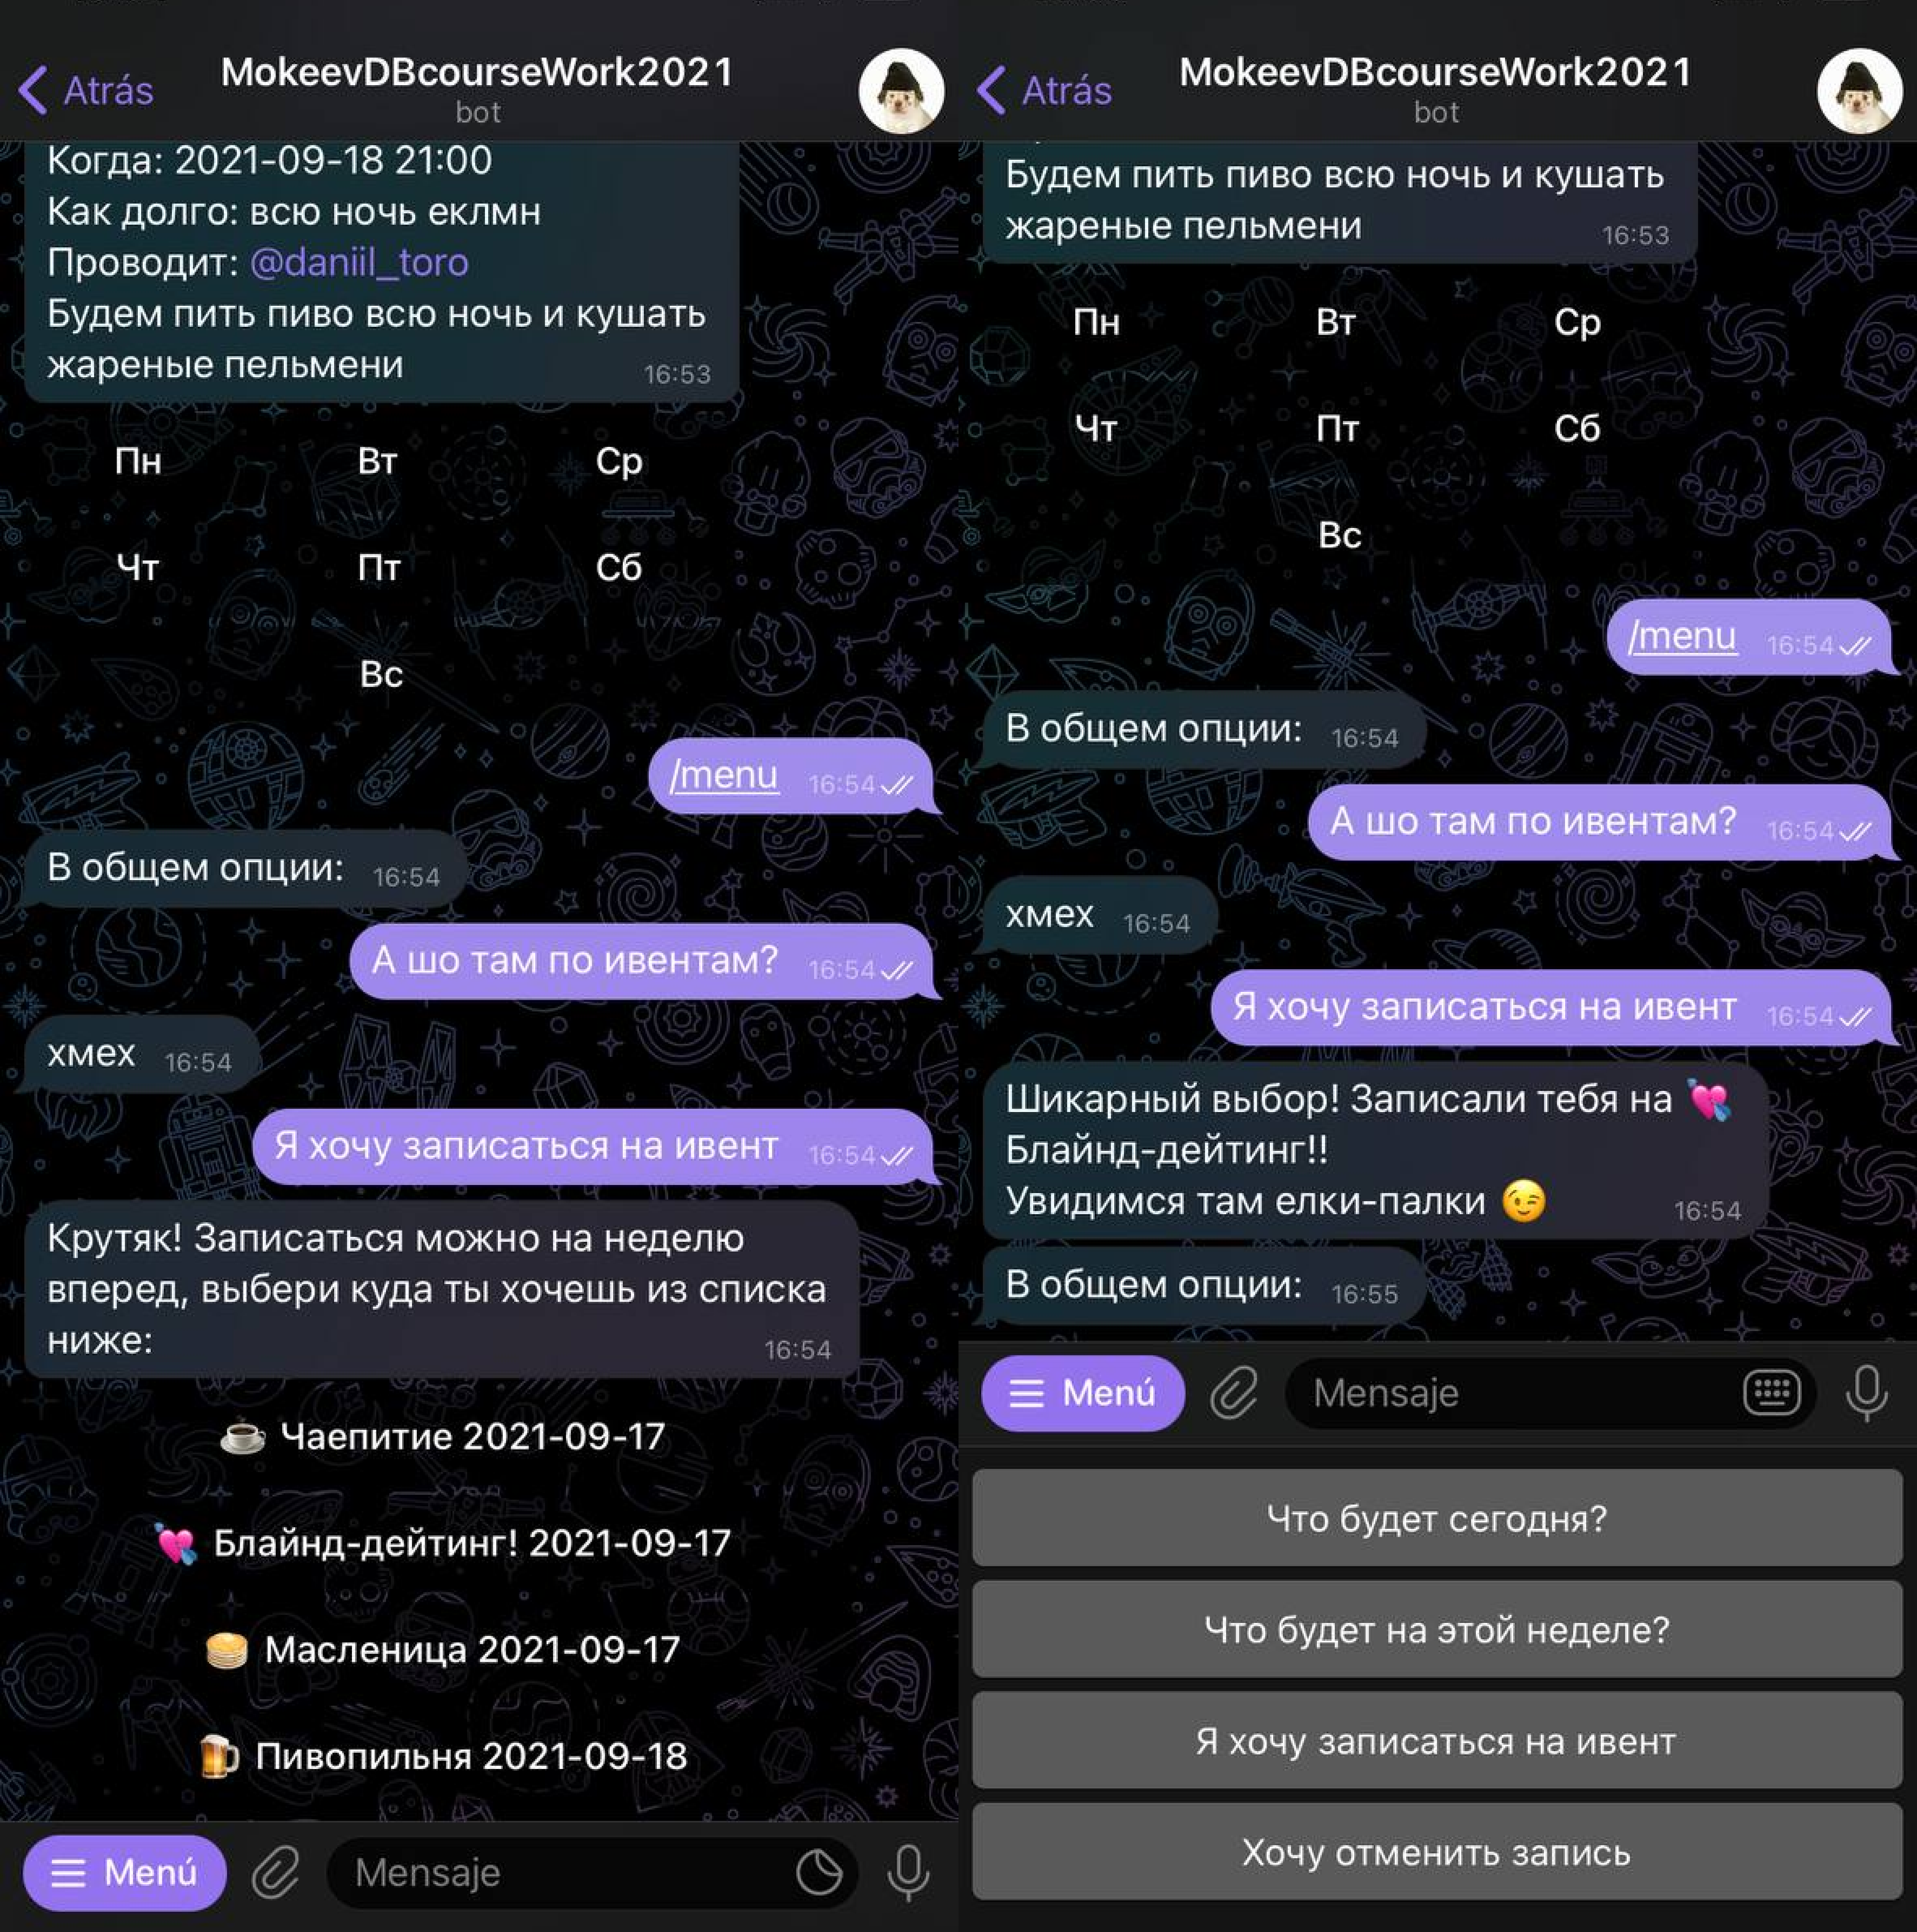
\includegraphics[scale=0.23]{RegEvent.png}
	\caption{Интерфейс регистрации на событие}
	\label{ris:regEvent}
\end{figure}

\begin{figure}[h]
	\centering
	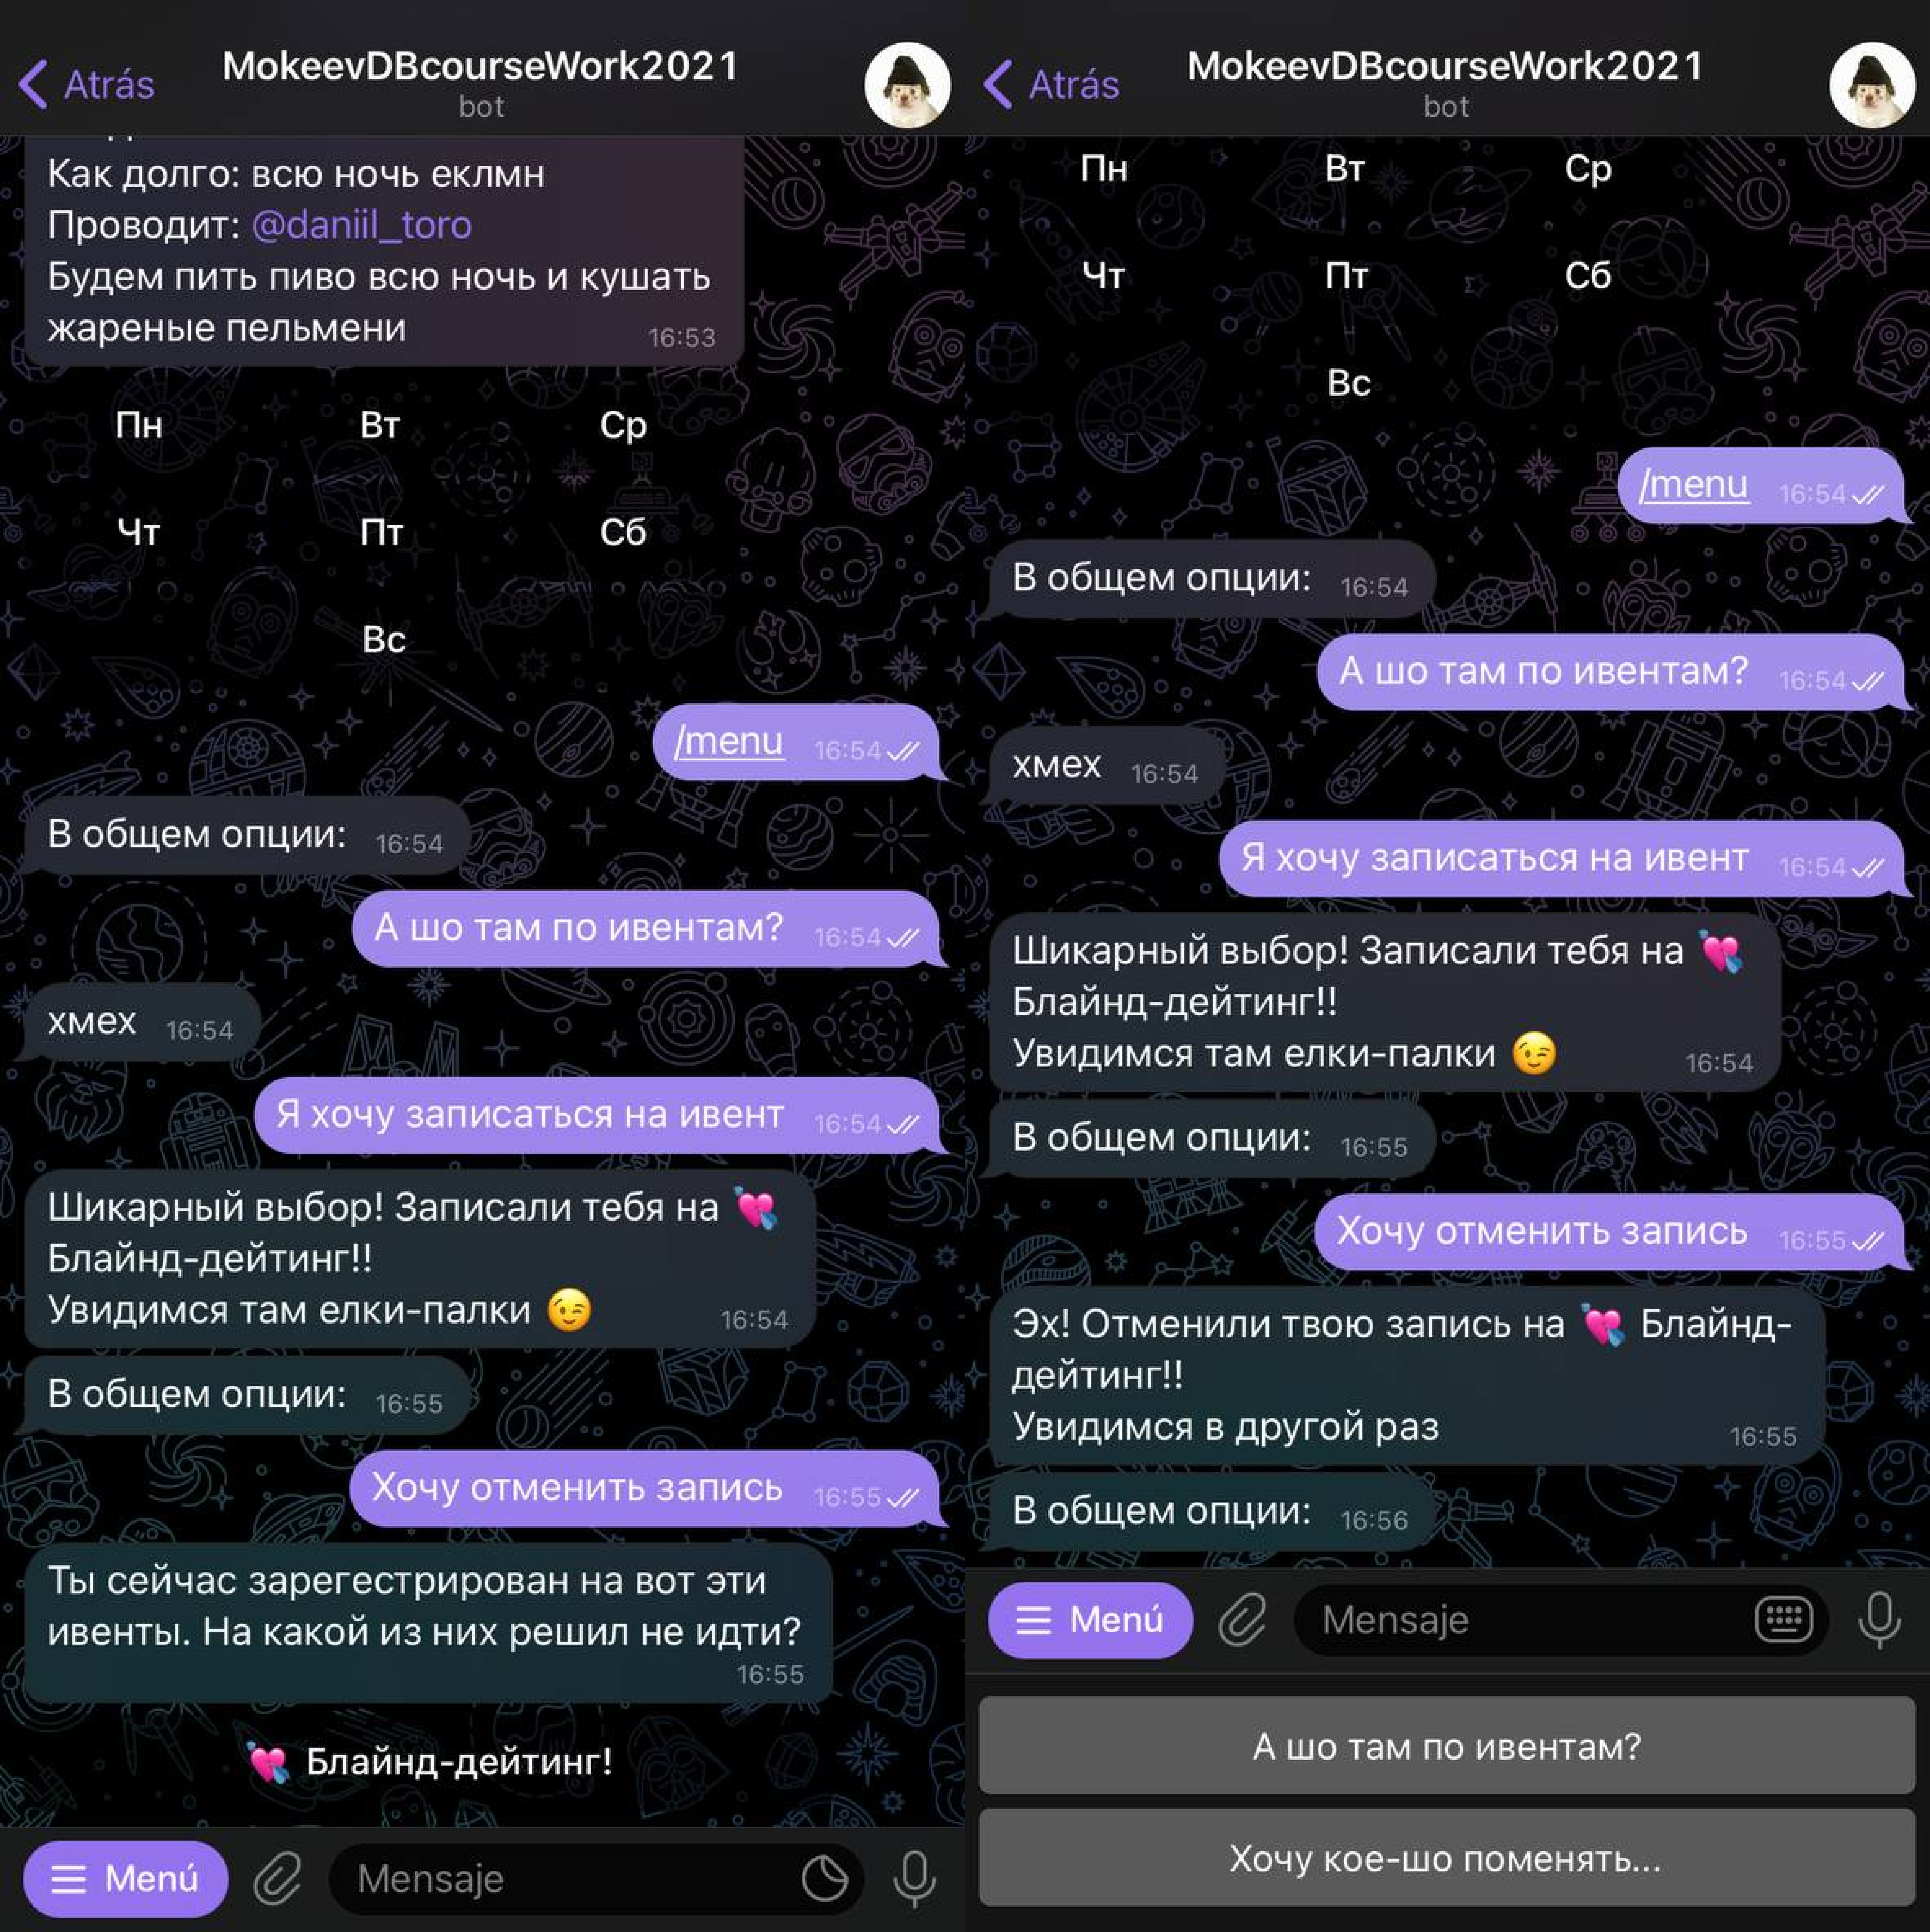
\includegraphics[scale=0.23]{Unreg.png}
	\caption{Интерфейс отмены регистрации на событие}
	\label{ris:unregEvent}
\end{figure}

 На рисунке \ref{ris:adminPass} показан интерфейс получения прав администратора и основное меню пользователя-администратора
 
\begin{figure}[h]
	\centering
	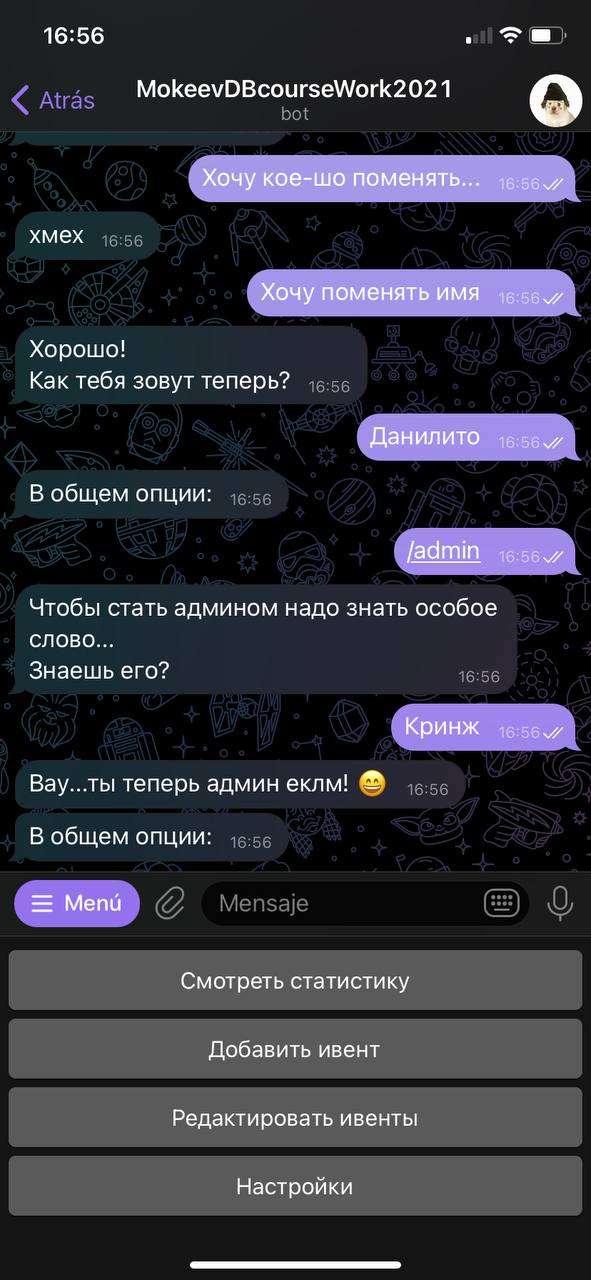
\includegraphics[scale=0.23]{adminChoice.jpeg}
	\caption{Получение прав администратора и основное меню}
	\label{ris:unregEvent}
\end{figure}

\section{Вывод}
\quad Были рассмотрены популярные СУБД и используемые алгоритмы работы чат-ботов, листинги реализованных классов для оформления таблиц базы данных. Был рассмотрен интерфейс приложения и его основные функции.

\addcontentsline{toc}{chapter}{Заключение}
\chapter*{Заключение}
\quad В результате выполнения курсового проекта была выполнена цель по разработке чат-бота на платформе мессенджера Telegram с подключением базы данных, задачей которого является обслуживание клиентов и сотрудников медицинских учреждений. Все запросы пользователей обрабатываются с использованием базы данных.
Были выполнены задачи поставленные во введении. Был выполнен анализ СУБД и анализ алгоритмов работы чат-ботов на платформе Telegram. Было спроектировано программное обеспечение, созданы схемы и диаграммы. Была спроектирована архитектура базы данных. Выбранные алгоритмы и структуры были реализованы в полной мере. Были произведены тестирование и отладка программного обеспечения.
В ходе данного курсового проекта были получены навыки создания чат-ботов на платформе Telegram, использования библиотеки Python Peewee для взаимодействия с СУБД SQLite.
\\

В результате проделанной работы:
\begin{itemize}
	\item формализована задача, определен необходимый функционал;
	\item проведён анализ инструментов, необходимых для проектирования и разработки приложения, в результате которого были выбраны СУБД SqlLight ORM Peewee;
	\item описана структуру базы данных, включая объекты, из которых она состоит;
	\item с помощью выбранных средств была создана платформа для управления событиями;
\end{itemize}

Цель работы достигнута, все задачи выполнены.



\addcontentsline{toc}{chapter}{Список использованной литературы}
\renewcommand{\bibname}{Список использованной литературы}
\begin{thebibliography}{2}

\bibitem{lection} Лекция № 3. Технологии баз данных — URL: \url{https://pandia.ru/text/78/475/50198.php}
(дата обращения: 15.06.2021).

\bibitem{subd} СУБД — URL:
\url{https://www.nic.ru/help/chto-takoe-subd\_8580.html}
(дата обращения: 17.06.2021).

\bibitem{deit} Дейт К. Дж. Введение в системы баз данных. — 8-е изд. — М.: «Вильямс», 2006.

\bibitem{ierarh} Иерархическая СУБД [Электронный ресурс]. – Режим доступа:
\url{https: //www.tadviser:ru/index:php/}
(Дата обращения: 18.06.2021)

\bibitem{seti} Сетевые модели данных [Электронный ресурс]. – Режим доступа: \url{https://studopedia.ru/220751setevie\_modeli\_dannih.html}
(Дата обращения: 18.06.2021)

\bibitem{rel} Основные понятия реляционной модели данных [Электронный ресурс]. – Режим доступа: \url{https://studopedia:ru/220752osnovnie\_ponyatiya\_relyatsionnoy\_modeli\_dannih.html}
(Дата обращения: 18.06.2021)

\bibitem{gavr} Гаврилова Юлия Михайловна, лекции из курса “Базы данных, ИУ7, 3 курс” — 2019 г.

\bibitem{sqlite} Интернет-ресурс Logz.io – сравнение характеристик популярных СУБД [Электронный ресурс]. 
\url{https://logz.io/blog/relational-database-comparison/}
(Дата обращения: 01.05.2020).

\bibitem{telegram} Документация библиотеки работы с  Telegram API — Telebot [Электронный ресурс]. – Режим доступа: URL
\url{https://core.telegram.org/bots/api}
(Дата обращения: 01.05.2020).

\bibitem{4} Документация Python 3.8.3 Режим доступа: URL:  
\url{https://docs.python.org/3/}
(Дата обращения: 01.05.2020).

\bibitem{5} Документация PyCharm [Электронный ресурс]. Режим доступа: URL 
\url{https://www.jetbrains.com/ru-ru/pycharm/documentation}
(Дата обращения: 01.05.2020).

\bibitem{6} ORM Peewee [Электронный ресурс]. – Режим доступа: URL: 
\url{http://docs.peewee-orm.com/en/latest/index.html}
(Дата обращения: 01.05.2020).

\bibitem{7} Документация СУБД SQLite [Электронный ресурс]. – Режим доступа: URL: 
\url{https://www.sqlite.org/index.html}
(Дата обращения: 01.05.2020).



\end{thebibliography}

\end{document}